\chapter{الجذور والكربينات وإعادات الترتيب}\label{ch:b3:radicals-carbenes}

تدافع زهرة البيرثروم عن نفسها بإسترات حمض الكريزانثيميك، وهي جزيئات
مبنية حول حلقة كربونية ثلاثية؛ ونظائرها الاصطناعية من بين
أكثر المبيدات الحشرية المنزلية استعمالًا. ويغلق الكيميائيون مثل هذه الحلقات في خطوة واحدة
بإضافة \omterm{def:b3:organometallic-bonding:carbene}{كربين} إلى رابطة مضاعفة: أي ذرة كربون لا يحيط بها إلا ستة إلكترونات،
اثنان منها غير مشتركين. ويعالج هذا الفصل الوسائط التفاعلية
التي لم يصادفها مجلدا السنة الأولى والسنة الثانية إلا عرضًا (الجذور المستعملة في
التخليق، والكربينات والنيترينات) وإعادات الترتيب التي تنتقل فيها مجموعة
إلى ذرة كربون أو نيتروجين أو أكسجين فقيرة بالإلكترونات، ومن بينها اثنتان
تصنعان مونومرَي النايلون-6 وبوليستر قابل للتحلل الحيوي من
الكيتون نفسه.

\begin{recall}
قدّم مجلد السنة الأولى الجذور والانشطار المتجانس والأسهم ذات نصف الرأس،
والكاتيونات الكربونية وإعادات ترتيبها، والمحبات للنواة والمجموعات المغادرة؛ وقدّم
مجلد السنة الثانية السلاسل الجذرية (البدء، والانتشار، والإنهاء، والبادئات
الجذرية)، والأحماض البيروكسية، واللاكتونات، واللاكتامات والإيمينات.
وعالج \cref{ch:b3:complex-kinetics} حركية السلاسل،
و\cref{ch:b3:organometallic-bonding} الكربينات بوصفها ربائط،
و\cref{ch:b3:many-electron-atoms} الحالات الأحادية والثلاثية، 
و\cref{ch:b3:rate-theories} مسلّمة هاموند.
\end{recall}

\begin{omfigure}
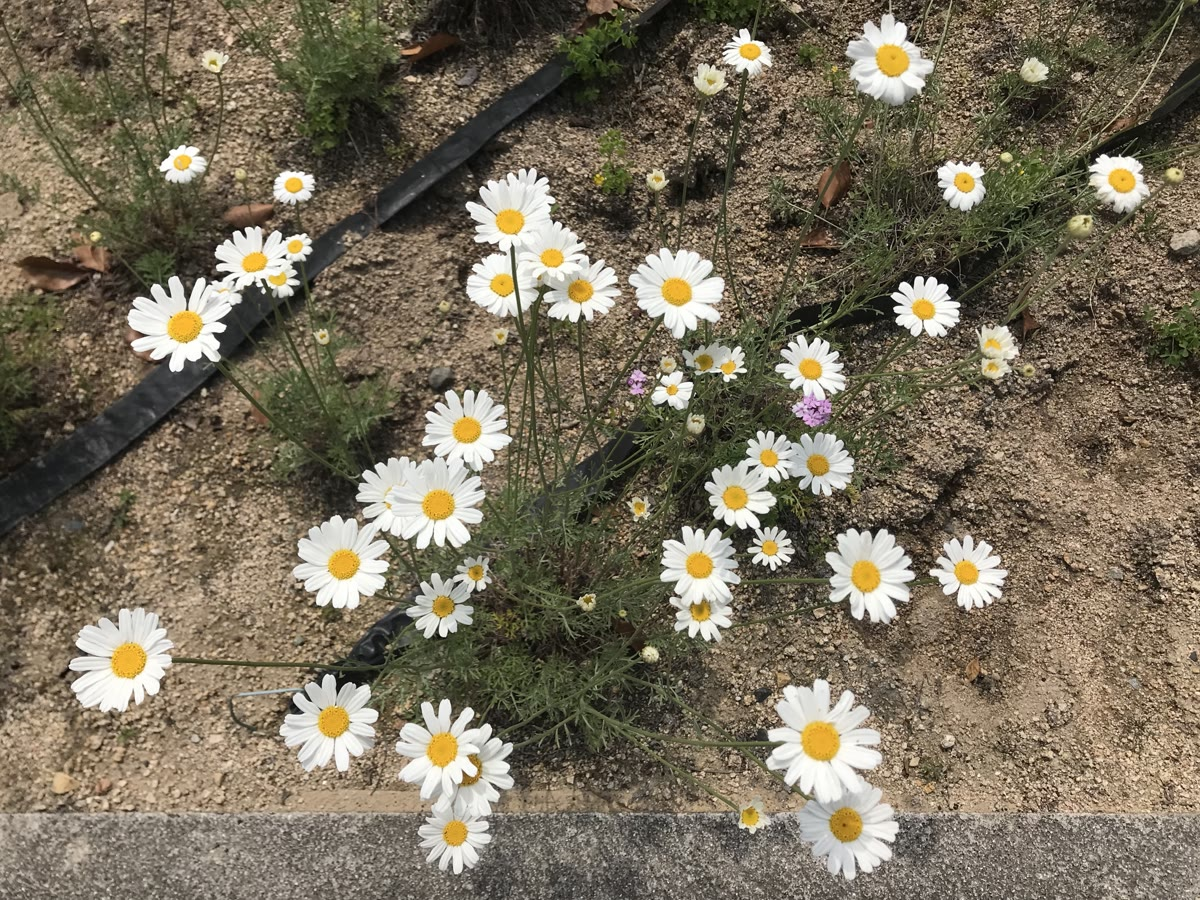
\includegraphics[width=0.48\linewidth]{images/book4/pyrethrum.jpg}

{\small أزهار البيرثروم. تحوي أزهارها البيريثرينات، وهي إسترات مبيدة للحشرات
لحمض سيكلوبروبان كربوكسيلي. الصورة: Soramimi، CC BY-SA 4.0.}
\end{omfigure}

\section{التفاعلات الجذرية المتسلسلة في التخليق}

يُقاس استقرار الجذر الكربوني بأنتالبي تفكك
الرابطة C--H التي كانت ستكوّنه: فكلما ضعفت الرابطة، ازداد
استقرار الجذر.

\begin{proposition}[أنتالبيات تفكك الروابط]\label{prop:b3:radicals-carbenes:bde}
تُستنتج أنتالبي تفكك الرابطة R--H عند \qty{298}{K} من أنتالبيات التكوين في
الطور الغازي: $\mathrm{BDE(R{-}H)} = \Delta_fH^\circ(\mathrm R^\bullet) + \Delta_fH^\circ(\mathrm H^\bullet) - \Delta_fH^\circ(\mathrm{RH})$.
\end{proposition}

\begin{proof}
للانشطار المتجانس $\mathrm{RH \to R^\bullet + H^\bullet}$، بحسب قانون هس، أنتالبي تفاعل تساوي أنتالبي تكوين النواتج
مطروحًا منها أنتالبي تكوين المتفاعل؛ وأنتالبي التفاعل هذه هي أنتالبي تفكك
الرابطة بحكم التعريف.
\end{proof}

\begin{omfigure}
% ledger: dfh4:CH3r, dfh4:C2H5r, dfh4:iC3H7r, dfh4:tC4H9r, dfh4:PhCH2r, dfh4:H, dfh:CH4_g, dfh:C2H6_g, dfh:C3H8_g, dfh4:iC4H10, dfh4:toluene_g
\begin{tikzpicture}
\begin{axis}[width=0.72\linewidth, height=5.2cm, ybar, bar width=16pt, ymin=350, ymax=450,
  xtick={1,2,3,4,5}, xticklabels={{$\ce{CH3-H}$}, {$\ce{C2H5-H}$}, {$\mathrm{(CH_3)_2CH{-}H}$}, {$\mathrm{(CH_3)_3C{-}H}$}, {$\ce{C6H5CH2-H}$}},
  x tick label style={font=\scriptsize}, ylabel={\foreignlanguage{arabic}{أنتالبي تفكك الرابطة \babelsublr{(\unit{kJ.mol^{-1}})}}},
  axis lines=left, tick label style={font=\scriptsize}, label style={font=\small},
  nodes near coords, nodes near coords style={font=\scriptsize, /pgf/number format/fixed, /pgf/number format/precision=0},
  enlarge x limits=0.15]
\addplot[fill=omDef!55, draw=omDef] table[x=i, y=bde] {figdata/out/bachelor-3-bde.dat};
\end{axis}
\end{tikzpicture}

{\small أنتالبيات تفكك الروابط C--H عند \qty{298}{K}، محسوبة من أنتالبيات التكوين
في الطور الغازي للجزيئات والجذور: الميثيل، والأولي،
والثانوي، والثالثي والبنزيلي. وتضعف الرابطة كلما كان الجذر المتكوّن
أكثر استبدالًا أو ترافقًا.}
\end{omfigure}

\begin{proposition}[انتقائية الهلجنة]\label{prop:b3:radicals-carbenes:halogenation-selectivity}
انتزاع الهيدروجين بذرة بروم أكثر انتقائية بكثير بين روابط C--H الأولية
والثانوية والثالثية من انتزاعه بذرة كلور.
\end{proposition}

\begin{proof}[تعليل]
مع $\mathrm{BDE(H{-}Cl)}$ أكبر من كل قيم C--H في الشكل و$\mathrm{BDE(H{-}Br)}$ أصغر منها،
يكون الانتزاع بالكلور ناشرًا للحرارة، وبالبروم ماصًا لها. وبحسب مسلّمة
هاموند (\cref{ch:b3:rate-theories}) تكون الحالة الانتقالية للكلور مبكرة،
شبيهة بالمتفاعلات، فلا تحس إلا قليلًا بالفرق بين الجذور المتكوّنة؛
أما حالة البروم فمتأخرة، شبيهة بالنواتج، وتتبع طاقة تنشيطها معظم
الفرق في أنتالبي التفكك، الذي يحوّله عامل بولتزمان إلى نسب سرعات كبيرة.
\end{proof}

يختزل هيدريد ثلاثي بوتيل القصدير هاليدات الألكيل بسلسلة: يأخذ جذر القصدير
الهالوجين، ويأخذ جذر الألكيل ذرة هيدروجين من الجزيء التالي من
الهيدريد، فيتكوّن جذر قصدير جديد. والسلسلة نفسها تزيل مجموعة هيدروكسي
بعد تحويلها إلى إستر ثيوكربونيلي (نزع الأكسجين وفق بارتون--ماكومبي)،
وتغلق الحلقات. وبقايا القصدير العضوي سامة وصعبة
الإزالة؛ ولذلك كثيرًا ما يحل اليوم محل هيدريد القصدير ثلاثي(ثلاثي ميثيل سيليل)السيلان وسيلانات
أخرى.

\begin{omfigure}
\begin{tikzpicture}[font=\small, >=Stealth]
  \node (a) at (-2.0,0) {$\mathrm{Bu_3Sn^\bullet}$};
  \node (b) at (2.0,0) {$\mathrm{R^\bullet}$};
  \draw[->, thick] (a) to[bend left=35] node[midway, above, font=\scriptsize] {$+\,$R--Br, $\ -\,\mathrm{Bu_3SnBr}$} (b);
  \draw[->, thick] (b) to[bend left=35] node[midway, below, font=\scriptsize] {$+\,\mathrm{Bu_3SnH}$, $\ -\,$R--H} (a);
  \node[font=\scriptsize, align=center, anchor=north] at (0,-1.5) {\foreignlanguage{arabic}{البدء:} AIBN $\xrightarrow{\Delta}$ 2 R$'^\bullet$ $+$ $\ce{N2}$; \ R$'^\bullet$ $+$ $\mathrm{Bu_3SnH}$ $\to$ R$'$H $+$ $\mathrm{Bu_3Sn^\bullet}$};
\end{tikzpicture}

{\small خطوات الانتشار في اختزال بروميد ألكيل بهيدريد القصدير.
كل R--Br مختزل يستهلك $\mathrm{Bu_3SnH}$ واحدًا ويعطي $\mathrm{Bu_3SnBr}$ واحدًا؛ وحاملا السلسلة
هما جذر القصدير وجذر الألكيل.}
\end{omfigure}

يُضاف بروميد الهيدروجين إلى الألكينات بسلسلة من النوع نفسه حين تكون البيروكسيدات
موجودة: تُضاف ذرة بروم إلى الطرف الأقل استبدالًا، فتعطي الجذر الأكثر
استقرارًا، الذي يأخذ بعد ذلك ذرة هيدروجين من HBr: إضافة مخالفة لماركوفنيكوف.

\section{التحلّقات الجذرية}

\begin{definition}[تحلّقات exo وendo]\label{def:b3:radicals-carbenes:cyclisation}
في \emph{تحلّق exo}\index{تحلق exo} تنتهي الرابطة المنكسرة (أو
الرابطة $\pi$ المهاجَمة) خارج الحلقة الجديدة؛ وفي \emph{تحلّق
endo}\index{تحلق endo}، داخلها.
\end{definition}

\begin{omfigure}
\begin{tikzpicture}[font=\scriptsize, >=Stealth]
  % hex-5-enyl radical: C1 radical, C5=C6
  \foreach \i/\a in {1/162, 2/234, 3/306, 4/18} { \coordinate (p\i) at (\a:0.9); }
  \coordinate (p5) at (90:0.95); \coordinate (p6) at (90:1.9);
  \draw[thick] (p1) -- (p2) -- (p3) -- (p4) -- (p5);
  \draw[thick, double, double distance=1.5pt] (p5) -- (p6);
  \node[anchor=east] at (p1) {$\bullet$\,1};
  \node[anchor=west] at (p5) {5}; \node[anchor=west] at (p6) {6};
  \draw[->, omMeth, thick] ($(p1)+(0.1,0.15)$) to[bend left=25] node[pos=0.45, below right, inner sep=1pt] {5-exo} ($(p5)+(-0.15,-0.05)$);
  \draw[->, omThm, thick, densely dashed] ($(p1)+(0,0.25)$) to[bend left=50] node[midway, left] {6-endo} ($(p6)+(-0.2,0)$);
  \node[font=\small, align=center] at (0,-1.6) {\foreignlanguage{arabic}{جذر هكس-5-إينيل}};
  \draw[->, thick] (1.6,0.3) -- (2.7,0.3) node[midway, above] {\foreignlanguage{arabic}{سريع}};
  \begin{scope}[xshift=4.0cm]
    \foreach \i/\a in {1/162, 2/234, 3/306, 4/18, 5/90} { \coordinate (q\i) at (\a:0.75); }
    \draw[thick] (q1) -- (q2) -- (q3) -- (q4) -- (q5) -- (q1);
    \draw[thick] (q5) -- ++(90:0.6) coordinate (q6);
    \node[anchor=south, inner sep=1pt] at (q6) {$\mathrm{{}^\bullet CH_2}$};
    \node[font=\small, align=center] at (0,-1.6) {\foreignlanguage{arabic}{جذر سيكلوبنتيل ميثيل}};
  \end{scope}
\end{tikzpicture}

{\small ينغلق جذر 5-هكسينيل بهجوم C1 على C5 (5-exo، بالأخضر): فللحلقة
الجديدة خمسة أعضاء وينتهي الجذر خارجها، على C6. والهجوم على C6
(6-endo، بالأحمر المتقطع) كان سيعطي جذر السيكلوهكسيل الثانوي الأكثر استقرارًا
لكنه أبطأ بكثير: فالسلسلة لا تستطيع أن تضع C1 على خط الاقتراب من C6 الذي
يقتضيه المدار $\pi^*$.}
\end{omfigure}

\begin{proposition}[قواعد بالدوين]\label{prop:b3:radicals-carbenes:baldwin}
من أجل إغلاقات الحلقات (وقد ثبتت تجريبيًا، مع تعليل
إلكتروني فراغي): عند كربون رباعي الأوجه (tet)، تكون من 3 إلى 7-exo مفضلة، و5 
و6-endo غير مفضلة؛ وعند كربون مثلثي (trig)، تكون من 3 إلى 7-exo مفضلة، ومن 3 إلى 5-endo
غير مفضلة، و6 و7-endo مفضلة؛ وعند كربون ثنائي (dig)، تكون 3 و4-exo
غير مفضلة، ومن 5 إلى 7-exo مفضلة، ومن 3 إلى 7-endo مفضلة.
\end{proposition}

التعليل هو زاوية الهجوم التي يحتاج إليها كل نوع من الروابط: من خلف
الرابطة عند كربون tet، وبزاوية نحو 107° على نظام $\pi$ مثلثي، وبزاوية
أضيق على رابطة ثلاثية؛ والسلسلة القصيرة لا تستطيع بلوغ تلك المواضع في
الحالات غير المفضلة.

\begin{definition}[الساعة الجذرية]\label{def:b3:radicals-carbenes:radical-clock}
\emph{الساعة الجذرية}\index{ساعة جذرية} جذر يعيد ترتيب نفسه
أحاديًا بثابت سرعة معلوم، مثل جذر 5-هكسينيل في
تحلّقه؛ ومنافسته مع مصيدة ثنائية الجزيئية تقيس ثابت سرعة
المصيدة، أو العكس.
\end{definition}

\begin{proposition}[حركية التنافس]\label{prop:b3:radicals-carbenes:clock}
إذا كان الجذر إما يتحلّق ($k_c$) وإما يُصطاد بهيدريد يُبقى بفائض عند
التركيز $[\mathrm{R_3SnH}]$ ($k_H$)، فإن نسبة النواتج هي
$[\text{الحلقي}]/[\text{المباشر}] = k_c/(k_H[\mathrm{R_3SnH}])$.
\end{proposition}

\begin{proof}
في كل لحظة يتكوّن الناتجان بالسرعتين $k_c[\mathrm R^\bullet]$ و$k_H[\mathrm{R_3SnH}][\mathrm R^\bullet]$. ونسبتهما
لا تتوقف على تركيز الجذر، الذي يتغير؛ ومع تركيز الهيدريد
الثابت، تضرب المكاملة على الزمن كلًّا منهما في المقدار نفسه
$\int[\mathrm R^\bullet]\,\dd t$، فتكون نسبة الناتجين هي نسبة ثابتي السرعة
مضروبة في $1/[\mathrm{R_3SnH}]$.
\end{proof}

\begin{omfigure}
\begin{tikzpicture}
\begin{axis}[name=a, width=0.47\linewidth, height=5.2cm, xmode=log, xmin=1e-3, xmax=1, ymin=0, ymax=1,
  axis lines=left, xlabel={\babelsublr{$[\mathrm{Bu_3SnH}]$ / \unit{mol.L^{-1}}}}, ylabel={\foreignlanguage{arabic}{النسبة المتحلّقة}},
  tick label style={font=\scriptsize}, label style={font=\small}]
\addplot[omDef, thick] table[x=c, y=fcyc] {figdata/out/bachelor-3-radical-clock.dat};
\end{axis}
\begin{axis}[at={(a.east)}, anchor=west, xshift=1.5cm, width=0.47\linewidth, height=5.2cm,
  xmin=0, xmax=1, ymin=0, ymax=11, axis lines=left,
  xlabel={\babelsublr{$[\mathrm{Bu_3SnH}]$ / \unit{mol.L^{-1}}}}, ylabel={\foreignlanguage{arabic}{[المباشر]/[الحلقي]}},
  tick label style={font=\scriptsize}, label style={font=\small}]
\addplot[omThm, thick] table[x=c, y=inv] {figdata/out/bachelor-3-radical-clock-b.dat};
\node[font=\scriptsize, anchor=west, omThm] at (axis cs:0.15,7.5) {\foreignlanguage{arabic}{الميل $k_H/k_c$}};
\end{axis}
\end{tikzpicture}

{\small ساعة 5-هكسينيل بثابتي سرعة نموذجيين $k_c = \qty{2.3e5}{s^{-1}}$ 
و$k_H = \qty{2.4e6}{L.mol^{-1}.s^{-1}}$. يسارًا: نسبة الميثيل سيكلوبنتان بين النواتج بدلالة
تركيز الهيدريد: النصف عند $k_c/k_H \approx \qty{0.1}{mol/L}$. يمينًا: النسبة العكسية مستقيم
يمر بالمبدأ، ميله $k_H/k_c$.}
\end{omfigure}

\begin{method}[تصميم اختزال جذري أو تحلّق]\label{met:b3:radicals-carbenes:radical-chain}
\begin{enumerate}
  \item من أجل اختزال بسيط، أبقِ مانح الهيدروجين مركّزًا (نحو
        \qty{0.1}{mol/L} أو أكثر) بحيث يُصطاد الجذر قبل أن يعيد ترتيب نفسه.
  \item من أجل تحلّق، أبقِ المانح ممددًا، أو أضفه ببطء، بحيث
        يتحلّق الجذر أولًا: اختر $[\text{المانح}] \ll k_c/k_H$.
  \item اختر بادئًا يكون عمر النصف له عند درجة حرارة التفاعل من
        رتبة زمن التفاعل (AIBN قرب \qty{80}{\celsius})، وأضفه على دفعات عند
        الحاجة.
  \item فضّل سيلانًا أو مانحًا آخر خاليًا من القصدير، وأزل الأكسجين، الذي يصطاد
        الجذور الكربونية.
\end{enumerate}
\end{method}

\begin{inthelab}[الإضافة البطيئة بمضخة محقنة]
لإبقاء كاشف ممددًا طوال التفاعل، يُعبّأ محلوله في
محقنة محكمة الإغلاق للغاز ويُضاف عبر حاجز بمضخة محقنة على مدى عدة
ساعات، إلى محلول الركيزة الذي يغلي مع التقطير الارتدادي تحت النيتروجين. فيبقى
تركيز الكاشف قرب قيمته المستقرة المنخفضة، التي تحددها
سرعة الإضافة وسرعة استهلاكه.
\end{inthelab}

\section{الكربينات}

\begin{definition}[الكربينات الأحادية والثلاثية]\label{def:b3:radicals-carbenes:carbene-states}
\emph{الكربين الأحادي}\index{كربين أحادي} إلكتروناه غير الرابطين
مزدوجان في مدار واحد، هجين $sp^2$، ومداره p فارغ؛ 
و\emph{الكربين الثلاثي}\index{كربين ثلاثي} إلكتروناه منفردان، واحد في كل
مدار، بسبينين متوازيين.
\end{definition}

\begin{omfigure}
\begin{tikzpicture}[font=\small]
  \node[align=center] at (0,0) {\foreignlanguage{arabic}{أحادي}\\[2pt] $sp^2$ \ \ p\\ \omorbs{ud,}};
  \node[align=center] at (4.2,0) {\foreignlanguage{arabic}{ثلاثي}\\[2pt] $sp^2$ \ \ p\\ \omorbs{u,u}};
  \node[font=\scriptsize, align=center] at (0,-1.3) {\foreignlanguage{arabic}{محب للإلكترونات، p فارغ،}\\ \foreignlanguage{arabic}{ومحب للنواة، زوج حر}};
  \node[font=\scriptsize, align=center] at (4.2,-1.3) {\foreignlanguage{arabic}{ثنائي جذر}};
\end{tikzpicture}

{\small إشغال المدارين غير الرابطين في \omterm{def:b3:organometallic-bonding:carbene}{الكربين} بالإلكترونات. \omterm{def:b3:many-electron-atoms:singlet-triplet}{الحالة
الثلاثية} هي الحالة الأساسية للجزيء $\ce{CH2}$؛ والمستبدلات المانحة $\pi$ (Cl، OR، $\mathrm{NR_2}$) ترفع
المدار p وتجعل \omterm{def:b3:many-electron-atoms:singlet-triplet}{الحالة الأحادية} هي الأساسية، كما في ثنائي كلوروكربين.}
\end{omfigure}

تُصنع الكربينات بفقد ثنائي النيتروجين من مركب ديازو (بالحرارة أو الضوء
أو بحفاز فلزي)، أو بالحذف $\alpha$ (يعطي الكلوروفورم مع قاعدة قوية
$\ce{CCl3-}$، الذي يفقد الكلوريد فيصير $\ce{CCl2}$)، أو تُتجنَّب كليًا باستعمال
\omterm{def:b3:radicals-carbenes:carbenoid}{كربينويد}.

\begin{definition}[الكربينويدات]\label{def:b3:radicals-carbenes:carbenoid}
\emph{الكربينويد}\index{كربينويد} نوع مرتبط بفلز ينقل
مجموعة كربينية كما يفعل \omterm{def:b3:organometallic-bonding:carbene}{الكربين} الحر، دون أن يتكوّن \omterm{def:b3:organometallic-bonding:carbene}{الكربين} الحر،
مثل يوديد يودوميثيل الزنك $\ce{ICH2ZnI}$ في تفاعل سيمونز--سميث.
\end{definition}

\begin{definition}[السيكلوبروبنة]\label{def:b3:radicals-carbenes:cyclopropanation}
\emph{السيكلوبروبنة}\index{سيكلوبروبنة} هي تكوين
سيكلوبروبان بإضافة \omterm{def:b3:organometallic-bonding:carbene}{كربين} أو \omterm{def:b3:radicals-carbenes:carbenoid}{كربينويد} إلى رابطة مضاعفة C=C.
\end{definition}

\begin{proposition}[اختبار سكيل]\label{prop:b3:radicals-carbenes:skell}
يُضاف \omterm{def:b3:radicals-carbenes:carbene-states}{الكربين الأحادي} إلى ألكين \textit{cis} أو \textit{trans} إضافة نوعية فراغيًا، محافظًا على
التشكيل النسبي؛ أما \omterm{def:b3:radicals-carbenes:carbene-states}{الكربين الثلاثي} فيعطي متماكبي السيكلوبروبان
الفراغيين كليهما.
\end{proposition}

\begin{proof}[تعليل]
يكوّن \omterm{def:b3:radicals-carbenes:carbene-states}{الكربين الأحادي} الرابطتين الجديدتين كلتيهما في خطوة متضافرة واحدة، دون وقت
للدوران. أما \omterm{def:b3:radicals-carbenes:carbene-states}{الكربين الثلاثي} فيكوّن رابطة واحدة أولًا، فيعطي ثنائي جذر 1،3 ثلاثيًا؛ ولا يستطيع
إلكتروناه المنفردان تكوين الرابطة الثانية حتى ينقلب سبين، وهذا
بطيء مقارنةً بالدوران حول الرابطة الأحادية C--C الباقية: فيختلط
التشكيل.
\end{proof}

\begin{omfigure}
\setchemfig{atom sep=1.8em}
\schemestart
\chemfig{H_3C-[:30]=[:0]-[:-30]CH_3}
\arrow{->[$\ce{CH2}$ أحادي]}[,1.6]
\chemfig{(<[:210]H_3C)-[:0](<[:330]CH_3)-[:120]-[:240]}
\schemestop
\par\medskip

{\small اختبار سكيل: \textit{cis}-بيوت-2-إين، ومجموعتا الميثيل فيه على الجانب نفسه، يعطي مع
\omterm{def:b3:radicals-carbenes:carbene-states}{كربين أحادي} \textit{cis}-1،2-ثنائي ميثيل سيكلوبروبان وحده (مجموعتا الميثيل كلتاهما على أوتاد،
على الوجه نفسه من الحلقة)؛ ومع \omterm{def:b3:radicals-carbenes:carbene-states}{كربين
ثلاثي} يظهر المتماكب \textit{trans} أيضًا.}
\end{omfigure}

تُدخَل الكربينات الأحادية أيضًا في روابط C--H. وتفكك كربوكسيلات الروديوم(II)
إسترات الديازو إلى كربينويدات روديوم تحوّل الألكينات إلى سيكلوبروبانات 
وتُدخَل في روابط C--H على نحو انتقائي، وعلى نحو انتقائي للمتماكبات المرآوية مع ربائط كيرالية.

\begin{definition}[النيترينات]\label{def:b3:radicals-carbenes:nitrene}
\emph{النيترين}\index{نيترين} $\mathrm{R{-}\ddot N}$ هو نظير \omterm{def:b3:organometallic-bonding:carbene}{الكربين} النيتروجيني، أي ذرة
نيتروجين متعادلة لا يحيط بها إلا ستة إلكترونات، تتكوّن مثلًا بفقد
ثنائي النيتروجين من أزيد.
\end{definition}

\section{إعادات الترتيب نحو كربون فقير بالإلكترونات}

\begin{definition}[الانزياح 1،2]\label{def:b3:radicals-carbenes:shift}
\emph{الانزياح 1،2}\index{انزياح 1،2} هو هجرة مجموعة، مع زوج
ارتباطها، من ذرة إلى الذرة المجاورة الفقيرة بالإلكترونات.
\end{definition}

في انزياح فاغنر--ميرفاين تنتقل مجموعة ألكيل أو هيدريد إلى كاتيون كربوني
مجاور، فتعطي كاتيونًا أكثر استقرارًا: وهي إعادات ترتيب الكاتيونات الكربونية في
مجلد السنة الأولى، وقد سُمّيت آليتها الآن. وتعيد الطبيعة تشكيل الهياكل التربينية
بسلاسل متعاقبة من هذه الانزياحات.

\begin{definition}[إعادة ترتيب البيناكول]\label{def:b3:radicals-carbenes:pinacol}
\emph{إعادة ترتيب البيناكول}\index{إعادة ترتيب البيناكول} تحوّل ثنائي ول 1،2،
في وسط حمضي، إلى كيتون أو ألدهيد: تغادر مجموعة هيدروكسي في صورة ماء،
وتنتقل مجموعة على الكربون المجاور إلى الكاتيون، ويفقد الكاتيون المتكوّن،
المستقر بالأكسجين الباقي، بروتونًا.
\end{definition}

\begin{definition}[القابلية للهجرة]\label{def:b3:radicals-carbenes:migratory}
\emph{القابلية للهجرة}\index{قابلية للهجرة} لمجموعة هي ميلها
النسبي إلى الانتقال في \omterm{def:b3:radicals-carbenes:shift}{انزياح 1،2} إلى مركز فقير بالإلكترونات.
\end{definition}

المجموعات التي تحمل الشحنة الموجبة جيدًا في أثناء الانزياح تهاجر أفضل: الهيدريد،
والأريل والألكيل الثالثي قبل الثانوي والأولي والميثيل. فالبيناكول،
$\mathrm{(CH_3)_2C(OH){-}C(OH)(CH_3)_2}$، يعطي البيناكولون، أي 3،3-ثنائي ميثيل بوتان-2-ون.

\begin{method}[التنبؤ بناتج إعادة ترتيب]\label{met:b3:radicals-carbenes:rearrangement}
\begin{enumerate}
  \item أوجد الذرة الفقيرة بالإلكترونات المتكوّنة (كاتيون، نيترينيوم، أكسجين
        بيروكسيد منشَّط، \omterm{def:b3:organometallic-bonding:carbene}{كربين} أو \omterm{def:b3:radicals-carbenes:nitrene}{نيترين}) والمجموعة المغادرة التي
        تكوّنها.
  \item عدّد المجموعات على الذرة المجاورة التي يمكن أن تنتقل؛ وحين تكون
        الهندسة ثابتة (الأوكسيمات)، لا يستطيع ذلك إلا المجموعة الواقعة في وضع anti من المجموعة المغادرة.
  \item وإلا فاختر بحسب \omterm{def:b3:radicals-carbenes:migratory}{القابلية للهجرة}، أو بحسب المجموعة التي تكوّن الكاتيون الأكثر
        استقرارًا حيث تغادر.
  \item انقل المجموعة مع الاحتفاظ بتشكيلها، ثم أكمل
        الآلية (فقد بروتون، إضافة ماء).
\end{enumerate}
\end{method}

\section{إعادات الترتيب نحو نيتروجين وأكسجين فقيرين بالإلكترونات}

\begin{definition}[إعادة ترتيب بكمان]\label{def:b3:radicals-carbenes:beckmann}
\emph{إعادة ترتيب بكمان}\index{إعادة ترتيب بكمان} تحوّل الأوكسيم،
في حمض قوي، إلى أميد: تغادر مجموعة الهيدروكسي، المنشَّطة مجموعةً مغادرة،
بينما تهاجر المجموعة الواقعة في وضع anti منها من الكربون إلى النيتروجين؛ ويُضاف الماء
إلى أيون النتريليوم المتكوّن، ويعطي التصاوغ الأميد.
\end{definition}

\begin{proposition}[الهجرة من وضع anti]\label{prop:b3:radicals-carbenes:beckmann-anti}
في \omterm{def:b3:radicals-carbenes:beckmann}{إعادة ترتيب بكمان} تكون المجموعة المهاجرة هي الواقعة في وضع anti من
المجموعة المغادرة على النيتروجين.
\end{proposition}

\begin{proof}[تعليل]
يهاجم الزوج الرابط المهاجر النيتروجين من خلف الرابطة N--O، كما في
استبدال $\mathrm S_\mathrm N2$؛ ولا تكون رابطة أي مجموعة مصطفة مع
المدار $\sigma^*$ للرابطة N--O إلا المجموعة الواقعة في وضع anti من الأكسجين. والخطوة متضافرة مع مغادرة المجموعة المغادرة،
فلا يتكوّن أيون نيترينيوم حر يمكنه أن يختار خلاف ذلك.
\end{proof}

\begin{omfigure}
\setchemfig{atom sep=1.9em}
\schemestart
\chemfig{*6(-----(=N-[:30]OH)-)}
\arrow{->[$\ce{H2SO4}$ (أوليوم)][بكمان]}[,1.8]
\chemfig{*7(---N(-[:-90]H)-(=O)---)}
\schemestop
\par\medskip
\schemestart
\chemfig{*6(-----(=O)-)}
\arrow{->[حمض بيروكسي][باير--فيليغر]}[,1.8]
\chemfig{*7(-----O-(=O)-)}
\schemestop

{\small توسيعان حلقيان للسيكلوهكسانون. في الأعلى: يعيد أوكسيمه ترتيب نفسه في
الأوليوم إلى الكابرولاكتام (أزيبان-2-ون)، مونومر النايلون-6، فيدخل النيتروجين
الحلقة. في الأسفل: يُدخل حمض بيروكسي ذرة أكسجين بجوار مجموعة
الكربونيل، فيعطي $\varepsilon$-كابرولاكتون (أوكسيبان-2-ون).}
\end{omfigure}

\begin{definition}[أكسدة باير--فيليغر]\label{def:b3:radicals-carbenes:baeyer}
\emph{أكسدة باير--فيليغر}\index{أكسدة باير--فيليغر} تحوّل
الكيتون إلى إستر، أو الكيتون الحلقي إلى لاكتون، بحمض بيروكسي: يُضاف
الحمض البيروكسي إلى مجموعة الكربونيل، ثم تهاجر مجموعة على كربون الكربونيل
إلى أقرب أكسجين بيروكسيدي بينما يغادر كربوكسيلات.
\end{definition}

\begin{proposition}[الانتقائية الموضعية في أكسدة باير--فيليغر]\label{prop:b3:radicals-carbenes:bv-retention}
في \omterm{def:b3:radicals-carbenes:baeyer}{أكسدة باير--فيليغر} تحتفظ المجموعة المهاجرة
بتشكيلها، وترتيب \omterm{def:b3:radicals-carbenes:migratory}{القابلية للهجرة} هو الألكيل الثالثي >
الألكيل الثانوي $\approx$ الأريل > الألكيل الأولي > الميثيل (وقد ثبت تجريبيًا).
\end{proposition}

\begin{proof}[تعليل]
تنتقل المجموعة مع زوج ارتباطها عبر وجه الكربون الذي تغادره
وتحط على الأكسجين من الجانب نفسه، فيُحفظ تشكيلها. وفي
الحالة الانتقالية تحمل المجموعة المهاجرة شحنة موجبة جزئية، يثبّتها
الاستبدال بالألكيل وترافق الأريل.
\end{proof}

\begin{definition}[الإيزوسيانات، وإعادتا ترتيب كورتيوس وهوفمان]\label{def:b3:radicals-carbenes:curtius}
\emph{الإيزوسيانات}\index{إيزوسيانات} مركب $\ce{R-N=C=O}$. وفي \emph{إعادة ترتيب كورتيوس}
\index{إعادة ترتيب كورتيوس} يفقد أزيد الأسيل ثنائي النيتروجين عند
التسخين بينما تنتقل المجموعة R من الكربون إلى النيتروجين، فيعطي إيزوسيانات؛
وفي \emph{إعادة ترتيب هوفمان}\index{إعادة ترتيب هوفمان} يعطي أميد أولي
يُعامل بالبروم وقاعدة الإيزوسيانات نفسه عبر
N-بروموأميد. ومع الماء يعطي الإيزوسيانات الأمين $\ce{RNH2}$ وثنائي أكسيد
الكربون؛ ومع كحول، كاربامات.
\end{definition}

\begin{definition}[الكيتينات وإعادة ترتيب فولف]\label{def:b3:radicals-carbenes:wolff}
\emph{الكيتين}\index{كيتين} مركب $\mathrm{R_2C{=}C{=}O}$. وفي \emph{إعادة ترتيب فولف}
\index{إعادة ترتيب فولف} يفقد ديازوكيتون $\alpha$ ثنائي النيتروجين
بينما تهاجر المجموعة التي على كربون الكربونيل، فيعطي كيتينًا، يضيف
الماء أو كحولًا أو أمينًا.
\end{definition}

\omterm{def:b3:radicals-carbenes:wolff}{إعادة ترتيب فولف} هي الخطوة الأساسية في الإطالة المتجانسة وفق أرندت--آيستيرت،
التي تطيل حمضًا كربوكسيليًا بذرة كربون واحدة: كلوريد الحمض، ثم
الديازوكيتون، ثم \omterm{def:b3:radicals-carbenes:wolff}{الكيتين}، ثم الحمض المتجانس الأطول.

\begin{safety}{\ghs[0.62cm]{GHS06}\ghs[0.62cm]{GHS08}\ghs[0.62cm]{GHS09}}
% ledger: ghs4:Bu3SnH, ghs4:diazomethane, ghs4:AIBN
هيدريد ثلاثي بوتيل القصدير: سام إذا ابتُلع، ضار على الجلد، يُتلف الأعضاء عند
التعرض المتكرر، شديد السمية للأحياء المائية؛ وتُجمع بقايا القصدير
على حدة. والديازوميثان غاز سام ومسرطن ومتفجر؛ ولا
يُذكر هنا إلا لكيميائه، ويُستبدل به عمليًا كواشف أكثر أمانًا
مثل ثلاثي ميثيل سيليل ديازوميثان. وAIBN ذاتي التفاعل عند التسخين.
\end{safety}

\begin{history}[جذر ما كان ينبغي أن يوجد، ونايلون]
في سنة 1900 حصل موزس غومبرغ، وهو يحاول صنع سداسي فينيل الإيثان، على محلول أصفر
يمتص الأكسجين واليود: جذر ثلاثي فينيل الميثيل، أول
جذر كربوني مستديم. وبعد نصف قرن، صارت \omterm{def:b3:radicals-carbenes:beckmann}{إعادة ترتيب بكمان} لأوكسيم
السيكلوهكسانون الطريق الصناعي إلى الكابرولاكتام، الذي يُبلمر بفتح
الحلقة إلى النايلون-6، وهو ليف ولدائن هندسية تُصنع على نطاق
واسع جدًا.
\end{history}

\section{تمارين}

\begin{exercise}[$\star$]\label{exo:b3:radicals-carbenes:1}
عند \qty{25}{\celsius} تكون التفاعليات النسبية لكل هيدروجين لروابط C--H الأولية والثانوية 
والثالثية $1 : 3.9 : 5.1$ إزاء ذرات الكلور و$1 : 82 : 1600$ إزاء
ذرات البروم (معطيات التمرين). احسب نسبتي 1- و2-هالوبروبان
المتكوّنين من البروبان في كل حالة.
\end{exercise}

\begin{exercise}[$\star$]\label{exo:b3:radicals-carbenes:2}
ما الحالة الأساسية للجزيء $\ce{CH2}$، وللجزيء $\ce{CCl2}$؟ وأيهما يُضاف إضافة نوعية فراغيًا إلى
\textit{trans}-بيوت-2-إين، وماذا يعطي؟
\end{exercise}

\begin{exercise}[$\star$]\label{exo:b3:radicals-carbenes:3}
أعطِ ناتج تفاعل سيمونز--سميث للمركب (\textit{Z})-هكس-3-إين.
\end{exercise}

\begin{exercise}[$\star$]\label{exo:b3:radicals-carbenes:4}
أعطِ نواتج \omterm{def:b3:radicals-carbenes:baeyer}{أكسدة باير--فيليغر} للسيكلوهكسانون 
وللأسيتوفينون.
\end{exercise}

\begin{exercise}[$\star\star$]\label{exo:b3:radicals-carbenes:5}
بمعطيات \cref{exo:b3:radicals-carbenes:1}، احسب نسب
الكلوريدين الأحاديين والبروميدين الأحاديين للمركب 2-ميثيل بروبان.
\end{exercise}

\begin{exercise}[$\star\star$]\label{exo:b3:radicals-carbenes:6}
تعطي \omterm{def:b3:radicals-carbenes:radical-clock}{ساعة جذرية} جديدة، مختزلة بتركيز $\qty{0.020}{mol/L}$ من $\mathrm{Bu_3SnH}$، ناتجًا معاد الترتيب أكثر بثلاث مرات
من الناتج غير المعاد الترتيب. ومع $k_H = \qty{2.4e6}{L.mol^{-1}.s^{-1}}$، أوجد ثابت سرعتها.
\end{exercise}

\begin{exercise}[$\star\star$]\label{exo:b3:radicals-carbenes:7}
صنّف وفق قواعد بالدوين هجوم جذر هكس-5-إينيل على C5 وعلى C6،
ثم قل هل كل من الإغلاقات التالية مفضل: 4-exo-tet، 5-endo-trig،
5-exo-dig، 3-exo-dig، 5-endo-dig.
\end{exercise}

\begin{exercise}[$\star\star$]\label{exo:b3:radicals-carbenes:8}
أعطِ ناتج \omterm{def:b3:radicals-carbenes:pinacol}{إعادة ترتيب البيناكول} للمركب 2،3-ثنائي فينيل بوتان-2،3-ثنائي ول،
وفسّر اختيار المجموعة المهاجرة.
\end{exercise}

\begin{exercise}[$\star\star$]\label{exo:b3:radicals-carbenes:9}
يُسخَّن أزيد البنزويل في التولوين، ثم يضاف الماء؛ وفي تجربة ثانية،
الإيثانول. أعطِ النواتج.
\end{exercise}

\begin{exercise}[$\star\star\star$]\label{exo:b3:radicals-carbenes:10}
مع $\mathrm{BDE(H{-}Cl)} = \qty{432}{kJ/mol}$ و$\mathrm{BDE(H{-}Br)} = \qty{366}{kJ/mol}$ (معطيات التمرين) وقيم C--H في
شكل الفصل، احسب $\Delta H$ لانتزاع هيدروجين أولي وهيدروجين ثالثي
بكل ذرة هالوجين، واستعمل مسلّمة هاموند لتفسير
انتقائيات \cref{exo:b3:radicals-carbenes:1}.
\end{exercise}

\begin{exercise}[$\star\star\star$]\label{exo:b3:radicals-carbenes:11}
أعطِ نواتج بكمان للأوكسيمين، \textit{E} و\textit{Z}، للمركب 2-ميثيل سيكلوهكسانون،
وفسّر لماذا تختلف، بينما تعطي \omterm{def:b3:radicals-carbenes:baeyer}{أكسدة باير--فيليغر} لهذا
الكيتون لاكتونًا رئيسيًا واحدًا.
\end{exercise}

\begin{exercise}[$\star\star\star$]\label{exo:b3:radicals-carbenes:12}
بالساعة النموذجية في الفصل، احسب النسبة المتحلّقة عند $[\mathrm{Bu_3SnH}] = 0.010$،
و0.10 و\qty{1.0}{mol/L}. وأي تركيز للهيدريد يعطي 95\,\% من الناتج المتحلّق، وكيف
يمكن الحفاظ عليه؟
\end{exercise}

\section{مسألة: حلقتان من السيكلوهكسانون}

\begin{problem}[{مسألة نهاية الأسبوع --- حلقتان من السيكلوهكسانون: الأوكسيم، 
وإعادة ترتيب بكمان إلى الكابرولاكتام، وأكسدة باير--فيليغر إلى
الكابرولاكتون، والانتقائية الموضعية في كلتيهما مع 2-ميثيل سيكلوهكسانون}]
\label{pb:b3:radicals-carbenes:1}
% ledger: aw:C, aw:H, aw:N, aw:O, aw:S
معطيات المسألة: يُحوَّل طن واحد من السيكلوهكسانون إلى أوكسيمه بمردود
98\,\%، ويُحوَّل الأوكسيم إلى كابرولاكتام بمردود 98\,\%؛ وتستعمل إعادة الترتيب
1.3 mol من حمض الكبريتيك (في صورة أوليوم) لكل مول من الأوكسيم، يُعادل في النهاية
بالأمونيا إلى كبريتات الأمونيوم.

\medskip\noindent\textbf{الجزء الأول --- الأوكسيم.}
\begin{enumerate}
  \item اكتب تكوّن أوكسيم السيكلوهكسانون من الهيدروكسيل أمين.
  \item لماذا يُجرى قرب pH بين 4 و5؟
  \item هل لأوكسيم السيكلوهكسانون متماكبات \textit{E} و\textit{Z}؟ لماذا؟
  \item ارسم الأوكسيمين \textit{E} و\textit{Z} للمركب 2-ميثيل سيكلوهكسانون.
  \item لماذا لا يتحول هذان الأوكسيمان أحدهما إلى الآخر إلا ببطء؟
\end{enumerate}

\medskip\noindent\textbf{الجزء الثاني --- \omterm{def:b3:radicals-carbenes:beckmann}{إعادة ترتيب بكمان}.}
\begin{enumerate}[resume]
  \item ماذا يفعل الحمض بالأوكسيم؟
  \item أي رابطة تهاجر، ولماذا تجعل الحلقة أكبر؟
  \item أي وسيط يهاجمه الماء؟
  \item اكتب المعادلة الإجمالية، من الأوكسيم إلى الكابرولاكتام.
  \item سمِّ الناتج وارسمه، والبوليمر المصنوع منه.
  \item احسب الكتلتين الموليتين للسيكلوهكسانون والكابرولاكتام.
  \item احسب كتلة الكابرولاكتام من طن واحد من السيكلوهكسانون.
  \item احسب كتلة كبريتات الأمونيوم المصنوعة معه.
\end{enumerate}

\medskip\noindent\textbf{الجزء الثالث --- \omterm{def:b3:radicals-carbenes:baeyer}{أكسدة باير--فيليغر}.}
\begin{enumerate}[resume]
  \item اكتب أكسدة السيكلوهكسانون بحمض بيروكسي $\ce{RCO3H}$.
  \item أعطِ الوسيط المتكوّن بإضافة الحمض البيروكسي.
  \item أي مجموعة تهاجر، وما المجموعة المغادرة؟
  \item سمِّ اللاكتون والبوليمر الذي يعطيه.
  \item لماذا يمكن أن يحل بيروكسيد الهيدروجين مع حفاز محل الحمض البيروكسي في
        عملية أنظف؟
\end{enumerate}

\medskip\noindent\textbf{الجزء الرابع --- 2-ميثيل سيكلوهكسانون.}
\begin{enumerate}[resume]
  \item أي ذرة كربون تهاجر في \omterm{def:b3:radicals-carbenes:baeyer}{أكسدة باير--فيليغر} له، وأي لاكتون يتكوّن؟
  \item هل يُحفظ تشكيل تلك الذرة؟
  \item أي لاكتام يعطيه الأوكسيم \textit{E} (المجموعة OH في وضع anti من الكربون الحامل للميثيل)؟
  \item أي لاكتام يعطيه الأوكسيم \textit{Z}؟
  \item ما الذي يحدد الانتقائية الموضعية في كل تفاعل؟
  \item لماذا يخلو السيكلوهكسانون نفسه من هذه المشكلات؟
  \item اذكر النتيجة: كتلة الكابرولاكتام من طن واحد من السيكلوهكسانون.
\end{enumerate}
\end{problem}
